\chapter{Elitzur-Vaidman Bomb Detection Algorithm}
\section{The Quantum Zeno Effect}

Suppose we have a qubit in the state $\ket{0}$, and we want to put it into the $\ket{1}$ state without using unitary transformations. For some small $\epsilon$, we can measure the qubit in a basis that's rotated from $\{\ket{0}, \ket{1}\}$ by an angle $\epsilon$. The probability of getting the qubit moved by $\epsilon$ increases as $\epsilon$ decreases.
\begin{align*}
P(\ket{v}) &= |\braket{0|v}|^2 = |\cos (\epsilon)|^2 \approx 1 - \epsilon^2 \quad && \text{where } \ket{v} = \cos(\epsilon) \ket{0} + \sin(\epsilon)\ket{1} \\
P(\ket{w}) &= |\braket{0|w}|^2 = |\sin (\epsilon)|^2 \approx \epsilon^2 \quad && \text{where } \ket{w} = -\sin(\epsilon) \ket{0} + \cos(\epsilon)\ket{1}
\end{align*}

So, by repeating this process $\approx 1/\epsilon$ times and rotating the measurement basis by an additional angle $\epsilon$ each time, we can slowly drag the qubit from $\ket{0}$ to $\ket{1}$. What's the likelihood that we ever get a measurement outcome that wasn't the one we wanted? By the union bound, it's of order $(1/\epsilon) \times \epsilon^2 = \epsilon$, so it can be made arbitrarily small. This is called the \textbf{Quantum Zeno Effect}. (One of its conceptual discoverers was \textit{Alan Turing}.)

Another interesting variant of this effect is called the \textbf{Watched Pot Effect}. Suppose we want to keep a qubit at $\ket{0}$, but it keeps rotating toward $\ket{1}$ (i.e., it's drifting). If we keep measuring it in the $\{\ket{0}, \ket{1}\}$ basis every time the qubit has drifted by an angle $\epsilon$, then the probability of it jumping to $\ket{1}$ during any given measurement is only $\epsilon^2$. So, if we repeat the measurements $\approx 1/\epsilon$ times, the total probability that it ends up in $\ket{1}$ is only $\approx \epsilon$, even though it would have drifted to $\ket{1}$ with certainty had we not measured.

\section{The Problem}

We are given a device which can either be a working bomb or a dud. The device takes a quantum bit as input and produces an output.

If the device is a bomb, it performs a measurement on the qubit. If the outcome of the measurement is $1$, then the bomb explodes; otherwise, it does not explode.

If the device is a dud, then it does nothing — i.e., the output is the same as the input.

We wish to determine whether the device is a bomb or a dud \emph{without} exploding the bomb. The Elitzur–Vaidman Bomb Detection Algorithm proceeds as follows:

\subsection{Approach 1: Naive Approach}

We give the device, naively, the input of $\ket{0}$ and $\ket{1}$.
\begin{itemize} 
    \item \textbf{Case 1: Device is a Bomb} \\
    If we give the device input $\ket{0}$, then the output will also be $\ket{0}$ always, because the outcome of the measurement will be $\ket{0}$, so the bomb doesn't explode and returns $\ket{0}$.  
    If we give the device input $\ket{1}$, then upon measurement, the outcome will be $\ket{1}$ and the bomb explodes always.

    \item \textbf{Case 2: Device is a Dud} \\
    For the input $\ket{0}$, if the device is a dud, then the output is $\ket{0}$ since it performs no operation on the input.  
    For the input $\ket{1}$, if the device is a dud, then the output is $\ket{1}$ since it performs no operation on the input.
\end{itemize}

To summarize the above approach: giving input $\ket{0}$ is of no help, as it provides no information about the device. In both cases (bomb or dud), the output will be $\ket{0}$.  
Upon giving input $\ket{1}$, if the device is a dud, then the output will be $\ket{1}$; but if the device is a bomb, it will explode. Thus, it tells us whether the device is a bomb or a dud, but if it's a bomb, it explodes. Hence, this approach is not useful since we can never detect a working bomb.

\subsection{Approach 2: Quantum Superposition Approach}

Here, we use a Hadamard gate before and after the device. The circuit is shown in Figure~\ref{fig:elitzur-vaidman}.

\begin{figure}[ht]
    \centering
    \begin{quantikz}[wire types={q,c}]
        & \gate{H} & \meter{} \wire[d][1]{c} & \gate{H} & \meter{} \wire[d][1]{c} &\\
        &&&& &
    \end{quantikz}
    % 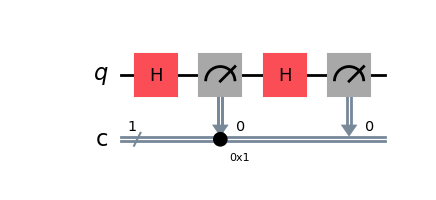
\includegraphics[width=0.5\textwidth]{Images/elitzur-vaidman.png}
    \caption{Elitzur-Vaidman Bomb Detection Algorithm}
    \label{fig:elitzur-vaidman}
\end{figure}

The first measurement occurs only if the device is a bomb.

\begin{itemize}
    \item \textbf{Case 1: Device is a Bomb} \\
    If we give input $\ket{0}$, then after passing through the Hadamard gate, the state becomes $\ket{+} = \frac{\ket{0} + \ket{1}}{\sqrt{2}}$.  
    As it passes through the device (which is a bomb), the device performs a measurement in the computational basis. The outcome will be $\ket{0}$ with probability $\frac{1}{2}$ and $\ket{1}$ with probability $\frac{1}{2}$.  
    In the case where the outcome is $\ket{0}$, the bomb does not explode, and the state then passes through another Hadamard gate, which transforms it back to $\ket{+}$.  
    Upon final measurement, we get $\ket{0}$ with probability $\frac{1}{2}$ and $\ket{1}$ with probability $\frac{1}{2}$.  
    In the case where the measurement outcome is $\ket{1}$, the bomb explodes.

    \item \textbf{Case 2: Device is a Dud} \\
    If we give input $\ket{0}$, then after passing through the Hadamard gate, the state becomes $\ket{+} = \frac{\ket{0} + \ket{1}}{\sqrt{2}}$.  
    As it passes through the device, which does nothing, the state remains $\ket{+}$.  
    Then, passing through the second Hadamard gate transforms $\ket{+}$ back to $\ket{0}$, and upon final measurement, we obtain the output $\ket{0}$.
\end{itemize}

To summarize this approach: suppose there are 1000 devices, of which 50\% are bombs and 50\% are duds. If we give input $\ket{0}$ to all the devices:  
- For all 500 duds, the output will be $\ket{0}$.  
- For the 500 bombs, due to the measurement in the device, 50\% (i.e., 250) will yield outcome $\ket{1}$ and explode, while the remaining 250 will yield outcome $\ket{0}$ and not explode.  

Those 250 non-exploded bombs with output $\ket{0}$ will then pass through a Hadamard gate, producing state $\ket{+}$, and upon final measurement, will give:  
- $\ket{0}$ with probability $\frac{1}{2}$  
- $\ket{1}$ with probability $\frac{1}{2}$  

Thus, from the 250 bombs that did not explode, 125 will output $\ket{1}$ and 125 will output $\ket{0}$.


    Thus, out of the 1000 devices, 250 bombs will explode. Among the remaining 750 devices, we will get an output of $\ket{0}$ from 625 of them — consisting of 500 duds and 125 bombs that did not explode — and an output of $\ket{1}$ from the remaining 125 devices.

Now, we are specifically interested in the cases where the output was $\ket{1}$ upon input $\ket{0}$. This is only possible if the device was a bomb that did not explode — since if it were a dud, the output would always have been $\ket{0}$. Thus, the 125 cases where the output was $\ket{1}$ upon input $\ket{0}$ correspond to bombs that did not explode.

So, out of the 500 bombs:
- 250 exploded,
- 125 did not explode and were successfully identified as working bombs,
- the remaining 125 did not explode but also could not be distinguished from duds.

Hence, we found 25\% of the working bombs without exploding them. Equivalently, we can say that:
- The probability of identifying a working bomb (without exploding it) among all the devices is $\frac{1}{8}$.
- Given that the device is a bomb, the probability of identifying it without explosion is $\frac{1}{4}$.

\textbf{What if the input had been $\ket{1}$?}  
The result would be similar. The only difference is that the output would be $\ket{1}$ for both duds and bombs that didn’t explode. Some bombs that didn't explode would instead give output $\ket{0}$, and those can then be identified as working bombs.

\textbf{Thus, we can find a working bomb with probability $\frac{1}{8}$ out of all the devices, or with probability $\frac{1}{4}$ given that the device is a bomb. However, note that in this process, half of the bombs (i.e., 250) exploded. Out of the remaining 250 bombs that did not explode, only half (125) were successfully identified, while the other half remained indistinguishable from duds.}


\subsection{Elitzur–Vaidman Bomb Detection Algorithm}

Recall that we are measuring in the orthonormal computational basis, i.e., $\ket{0}$ and $\ket{1}$. Consider the single-qubit gate $R^Y_{\theta}$, which is defined as:
\[
    R^Y_{\theta} = \begin{bmatrix}
        \cos\frac{\theta}{2} & -\sin\frac{\theta}{2} \\
        \sin\frac{\theta}{2} & \cos\frac{\theta}{2} \\
    \end{bmatrix}
\]
where $\theta$ is the angle of rotation. The $R^Y_{\theta}$ gate is a rotation gate about the Y-axis. It is a unitary gate and thus preserves the norm of the vector as well as inner products. It is also a Hermitian gate. Thus, $R^Y_{\theta}$ is self-inverse:
\[
    R^Y_{\theta} = (R^Y_{\theta})^{\dagger} = (R^Y_{\theta})^{-1}.
\]

The action of the $R^Y_{\theta}$ gate on the state $\ket{0}$ is as follows:
\[
    R^Y_{\theta} \ket{0} = 
    \begin{bmatrix}
        \cos\frac{\theta}{2} & -\sin\frac{\theta}{2} \\
        \sin\frac{\theta}{2} & \cos\frac{\theta}{2} \\
    \end{bmatrix}
    \begin{bmatrix}
        1 \\
        0 \\
    \end{bmatrix}
    =
    \begin{bmatrix}
        \cos\frac{\theta}{2} \\
        \sin\frac{\theta}{2} \\
    \end{bmatrix}
    = \cos\frac{\theta}{2}\ket{0} + \sin\frac{\theta}{2}\ket{1}
\]

Thus, upon measurement, the probability of getting $\ket{0}$ is $|\cos\frac{\theta}{2}|^2$ and the probability of getting $\ket{1}$ is $|\sin\frac{\theta}{2}|^2$. Hence, the $R^Y_{\theta}$ gate performs a rotation about the Y-axis by an angle $\theta$.

Clearly, for very small $\theta$, the probability of getting $\ket{0}$ is approximately $\cos^2 \frac{\theta}{2} \approx 1$.

The circuit for the Elitzur–Vaidman Bomb Detection Algorithm is shown in Figure~\ref{elitzur}.

\begin{figure}[ht]
    \centering
    \begin{quantikz}
        \lstick[1]{$\ket{0}$} & \gate{R_Y\left({\frac{\pi}{N}}\right)}\gategroup[1,steps=2,style={dashed,rounded corners, , inner xsep=2pt},background,label style={label position=above, anchor=south, yshift=-0.2cm}]{{\sc $N times$}} & \gate{Device} & \meter{}
    \end{quantikz}
    % 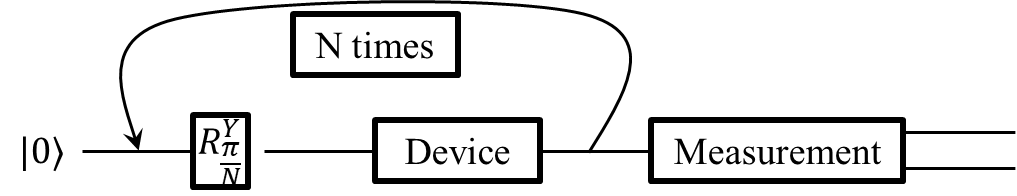
\includegraphics[width=0.8\textwidth]{Images/elitzur-vaidmanfinal.png}
    \caption{Elitzur–Vaidman Bomb Detection Algorithm}
    \label{elitzur}
\end{figure}

Thus, when we pass $\ket{0}$ through the $R^Y_{\theta}$ gate, the output will be $\cos\frac{\theta}{2}\ket{0} + \sin\frac{\theta}{2}\ket{1}$.

\begin{itemize}
    \item \textbf{Case 1: Device is a Dud} \\
    Since the device is a dud, it does nothing. After the first iteration, the state becomes:
    \[
        \cos\frac{\pi}{2N}\ket{0} + \sin\frac{\pi}{2N}\ket{1}.
    \]
    In the second iteration, we again apply the $R^Y_{\theta}$ gate:
    \[
        R_Y({\frac{\pi}{N}})
        \begin{bmatrix}
            \cos\frac{\pi}{2N} \\
            \sin\frac{\pi}{2N} \\
        \end{bmatrix}
        =
        \begin{bmatrix}
            \cos^2\frac{\pi}{2N} - \sin^2\frac{\pi}{2N} \\
            2\cos\frac{\pi}{2N} \sin\frac{\pi}{2N} \\
        \end{bmatrix}
        =
        \cos\frac{\pi}{N}\ket{0} + \sin\frac{\pi}{N}\ket{1}.
    \]

    Thus, after the second iteration, the output is $\cos\frac{\pi}{N}\ket{0} + \sin\frac{\pi}{N}\ket{1}$. Continuing this way, after the $k$-th iteration, the state becomes:
    \[
        \cos\frac{k\pi}{2N}\ket{0} + \sin\frac{k\pi}{2N}\ket{1}.
    \]
    Therefore, after the $N$-th iteration, the output will be:
    \[
        \cos\frac{\pi}{2}\ket{0} + \sin\frac{\pi}{2}\ket{1} = \ket{1}.
    \]
    Hence, for a dud device, the final output after $N$ steps is $\ket{1}$.

    \item \textbf{Case 2: Device is a Bomb} \\
    Since the device is a bomb, it performs a measurement. After the first application of $R^Y_{\theta}$, the state becomes:
    \[
        \cos\frac{\pi}{2N}\ket{0} + \sin\frac{\pi}{2N}\ket{1}.
    \]
    The bomb measures this state in the computational basis. The probability of getting $\ket{0}$ is $\cos^2\frac{\pi}{2N}$ and of getting $\ket{1}$ is $\sin^2\frac{\pi}{2N}$.

    Now, consider the case for very large $N$:
    \[
        \lim_{N \to \infty} \cos^2\frac{\pi}{2N} \approx \cos^2 0 = 1, \quad \lim_{N \to \infty} \sin^2\frac{\pi}{2N} \approx 0.
    \]
    Thus, the probability of the bomb exploding (i.e., measurement result $\ket{1}$) becomes vanishingly small.

    Therefore, with high probability, the output after the first measurement is $\ket{0}$, which is again passed through $R^Y_{\theta}$ in the second iteration. This process repeats identically for each of the $N$ iterations.

    After $N$ iterations, assuming the bomb hasn’t exploded (which is highly likely for large $N$), the final output will be $\ket{0}$.

    Hence, when the device is a bomb, the circuit either:
    \begin{itemize}
        \item outputs $\ket{0}$ with high probability, or
        \item explodes with very low probability (which decreases as $N$ increases).
    \end{itemize}

    Therefore, the probability of explosion is inversely proportional to the number of iterations $N$, and in the limit of large $N$, the device effectively acts as a measurement without disturbing the bomb.
\end{itemize}

    The probability that the bomb explodes after the first iteration is $\sin^2 \left( \frac{\pi}{2N} \right)$, and the probability that the bomb explodes after $N$ iterations is $\sin^{2N} \left( \frac{\pi}{2N} \right)$. 

This is because the explosion of the bomb is an independent event in each iteration. For independent events, we have:
\[
P(A \cap B \cap \ldots \cap Z) = P(A) \cdot P(B|A) \cdots P(Z|A,B,\ldots,Z) = P(A) \cdot P(B) \cdots P(Z),
\]
so the probability 
\[
P(\text{bomb explodes in 1st} \land \text{2nd} \land \ldots \land \text{$N$-th iteration}) = \left[\sin^2\left( \frac{\pi}{2N} \right)\right]^N = \sin^{2N}\left( \frac{\pi}{2N} \right).
\]

For very large $N$, we can use the small-angle approximation:
\[
\sin\left( \frac{\pi}{2N} \right) \approx \frac{\pi}{2N}.
\]
Hence, the probability of the bomb exploding after $N$ iterations is approximately:
\[
\left( \frac{\pi}{2N} \right)^{2N}.
\]

\begin{table}[ht]
    \centering
    \begin{tabular}{|c|c|}
        \hline
        $N$ & Probability of Bomb Exploding \\
        \hline
        2 & $0.25$ \\
        10 & $7.702 \times 10^{-17}$  \\
        20 & $6.105 \times 10^{-45}$ \\
        $\vdots$ & $\vdots$ \\
        500 & $1.409 \times 2^{-2503}$ \\
        \hline
    \end{tabular}
    \caption{Probability of bomb exploding after $N$ iterations}
    \label{tab:Prob}
\end{table}

As can be seen from Table~\ref{tab:Prob}, the probability of the bomb exploding after $N$ iterations drops rapidly for large $N$. Thus, the Elitzur–Vaidman Bomb Detection Algorithm is a very efficient method for detecting a working bomb without exploding it.







\chapterreferences
